\documentclass[journal]{IEEEtran}
\usepackage{amsmath,amssymb}
\usepackage{graphicx}
\usepackage{booktabs}
\usepackage{multirow}
\usepackage{xcolor}
\usepackage{url}
\usepackage[hidelinks]{hyperref}
\usepackage{cite}
\graphicspath{{figures/}}
\newcommand{\figw}{\columnwidth}

\begin{document}

\title{Leakage-Controlled Benchmarking of Fourteen Multimodal Fusion Architectures for Explainable Melanoma Classification from Dermoscopic Images and Clinical Metadata}

\author{Abdelrahman~Mohamed, Ahmed~Mohsen, Jana~Ahmed, and~Malak~Mohamed
\thanks{Manuscript received 17 May 2026; revised 24 November 2026.}
\thanks{The authors are with the University of Science and Technology, Zewail City, Giza, Egypt.}}

\markboth{Revised manuscript}{Mohamed \MakeLowercase{\textit{et al.}}: Leakage-Controlled Multimodal XAI for Melanoma Classification}

\maketitle

\begin{abstract}
Multimodal deep learning that fuses dermoscopic images with patient metadata is widely reported to improve melanoma detection, yet published comparisons rarely control for label leakage, rarely evaluate all architectures on an identical test set, and rarely test whether explanations are faithful to the model. We address all three gaps on the balanced ISIC-DICM-17K corpus (17,059 images). First, we show that the \emph{diagnosis-confirmation-type} field deterministically encodes the label for roughly one quarter of the corpus (every non-histopathological confirmation implies a benign lesion), and we remove it; a residual acquisition shortcut (dermoscope vignetting) is neutralised by counterfactual vignette augmentation. Second, we train fourteen fusion architectures, spanning early/late token fusion, cross-attention, bidirectional cross-attention, graph-attention, gated and bilinear fusion over nine visual backbones, under one shared protocol (fixed split, optimiser, augmentation, exponential moving average, eight-view test-time augmentation, temperature scaling) and evaluate them on the same 2,559 held-out images with bootstrap confidence intervals and Holm-corrected paired DeLong tests. ViT-B/16 early fusion ranks first (AUC 0.937, 95\% CI 0.929--0.945; balanced accuracy 0.861; ECE 0.036), but it is statistically indistinguishable from four other models (late-fusion ViT, MaxViT+GATv2, SegFormer-B5+LACA, DaViT+gated fusion); fusion \emph{depth} matters less than backbone pre-training quality. A validation-selected four-model ensemble raises AUC to 0.944 ($p<0.001$). Third, we expose a patient-level overlap in the community split (84\% of test images come from patients seen in training): on patient-disjoint images every model loses 0.07--0.10 AUC, although the ranking is preserved (Spearman $\rho=0.83$). Finally, we explain every model on the \emph{same} test cases and score explanations by deletion/insertion faithfulness against a random-map baseline and by lesion localisation. Integrated Gradients is the most faithful and most lesion-focused method (faithfulness gain over random 0.25; 45\% of attribution energy inside the lesion), significantly above random for all fourteen models, whereas Grad-CAM++ is the least faithful (0.10; Friedman $p<10^{-6}$). Grouped Shapley values and permutation importance agree across models (Kendall's $W=0.74$) that melanocytic status and age dominate metadata reliance.
We release all code, predictions and figures to support reproducible multimodal dermatology research.
\end{abstract}

\begin{IEEEkeywords}
Melanoma classification, multimodal fusion, explainable artificial intelligence, dermoscopy, clinical metadata, data leakage, shortcut learning, Vision Transformer, faithfulness evaluation, calibration.
\end{IEEEkeywords}

\section{Introduction}
\IEEEPARstart{S}{kin} cancer is one of the most prevalent and rapidly increasing forms of cancer worldwide, with melanoma considered the most aggressive subtype because of its high metastatic potential and mortality rate. More than 1.5 million new skin-cancer cases were estimated in 2022; an estimated 330,000 of these were melanomas, and almost 60,000 people died from the disease. Accurate melanoma detection nonetheless remains difficult because malignant lesions often closely resemble benign ones, and variations in texture, pigmentation, asymmetry and border irregularity complicate assessment even for experienced dermatologists.

Dermoscopy enables enhanced visualisation of subsurface lesion structures, and deep convolutional and Transformer networks trained on dermoscopic images now rival dermatologists on curated benchmarks \cite{esteva2017,haenssle2018}. Most such systems, however, rely exclusively on the image and ignore the structured clinical context, such as age, sex, anatomical site and lesion history, that clinicians routinely combine with visual inspection. Melanoma classification is therefore naturally a \emph{multimodal} problem, and a growing body of work fuses image features with metadata \cite{ahammed2025,aksoy2025}. How best to fuse the two modalities remains an open design question, and published comparisons are difficult to interpret for three reasons that motivate this study.

\textit{(i) Leakage through metadata.} Public dermoscopy metadata contain acquisition variables that are correlated with the label by construction. In ISIC-derived corpora, malignant ground truth is assigned only to biopsied lesions, so the \emph{diagnosis-confirmation} field reveals the label for every lesion confirmed by follow-up imaging or expert consensus. A model given this field learns the curation protocol, not dermatology, and its reported accuracy (and its SHAP explanations) are inflated accordingly. An earlier version of this work, like much of the literature, included this field.

\textit{(ii) Non-comparable evaluation.} Architectures are typically reported from separate experiments with different splits, preprocessing, training budgets and threshold rules, and without uncertainty estimates or paired significance tests, so small differences in AUC are routinely over-interpreted.

\textit{(iii) Unverified explanations.} Saliency maps are usually shown for a handful of cherry-picked images, each model on different images, with no test of whether the highlighted pixels actually drive the prediction \cite{adebayo2018}.

This paper makes the following contributions:
\begin{enumerate}
\item A \textbf{leakage audit} of ISIC-DICM-17K metadata, which identifies the confirmation-type field as a deterministic label proxy for $\approx$25\% of samples, dermoscope vignetting as an image-level acquisition shortcut, and an 84\% patient-level overlap between the community train and test splits.
\item A \textbf{controlled benchmark of fourteen multimodal architectures} spanning six fusion families and nine backbones, trained under one protocol and evaluated on the identical test set with bootstrap CIs, Holm-corrected paired DeLong tests, nine-metric composite ranking, calibration, decision-curve and subgroup analyses.
\item A \textbf{unified-case XAI evaluation}: every model is explained on the same test images with Grad-CAM, Grad-CAM++, Integrated Gradients, occlusion and attention roll-out; maps are scored by deletion/insertion faithfulness against a random baseline and by lesion localisation, and metadata reliance is quantified with grouped Shapley values and permutation importance.
\item Evidence-based \textbf{design guidance}: backbone pre-training quality dominates fusion mechanism, the five best models are statistically tied, and a small validation-selected ensemble is significantly better than any single model.
\end{enumerate}

\section{Review of Relevant Literature}
\subsection{Image-Only Models: Performance Without Context}
The earliest and most common approach to automated lesion classification feeds dermoscopic images alone into convolutional networks. Kassem \textit{et al.} \cite{kassem2020} achieved 94.92\% accuracy on an eight-class task with a fine-tuned GoogLeNet, and Ahmad \textit{et al.} \cite{ahmad2023} trained a CNN on 20,000 images, reaching over 90\% accuracy and an AUC of approximately 0.95. Both treat the image as the sole diagnostic input and ignore the patient-level information that dermatologists routinely use; melanoma risk varies substantially with age and anatomical site, so an image-only model must approximate these priors indirectly. Neither study offers a mechanism for explaining predictions. Mahmud \textit{et al.} \cite{mahmud2025} enhanced the Xception backbone (96.48\% on one dataset) and added Grad-CAM and saliency maps, a meaningful step toward transparency, but still disregarded patient data and used purely visual, post-hoc explanations.

\subsection{Explainability Methods: Varieties and Trade-offs}
\subsubsection{Post-hoc visual explanations}
Grad-CAM \cite{selvaraju2017} and Grad-CAM++ \cite{chattopadhay2018} weight convolutional activations by class-score gradients to produce coarse localisation heat-maps. Muduli \textit{et al.} \cite{muduli2025} integrated Grad-CAM into an attention-gated U-Net that jointly segments and classifies lesions (92.75\% accuracy on ISIC~2016), and Gamage \textit{et al.} \cite{gamage2024} combined U$^2$-Net lesion masking with Grad-CAM++ (98.37\% accuracy; 86.87\% clinician usability score). These methods are inexpensive and intuitive, but they explain \emph{where} a model looked, not \emph{why}, and they can be insensitive to the model parameters themselves \cite{adebayo2018}. Ruga \textit{et al.} \cite{ruga2026} paired Grad-CAM with SHAP \cite{lundberg2017} over handcrafted descriptors in the MultiExCam ensemble (AUC 0.91--0.98), bridging visual and quantitative interpretability at the cost of inference latency.

\subsubsection{Attention-based interpretability}
The Vision Transformer (ViT) \cite{dosovitskiy2021} processes an image as a sequence of patches whose self-attention weights can be visualised directly. ViT matches or outperforms CNNs when pre-trained on very large corpora but lacks convolutional inductive biases, so in dermatology it is most useful as a pre-trained backbone that is fine-tuned on domain data. Raw attention is not, however, a faithful attribution by itself; gradient-weighted roll-out is commonly used instead.

\subsubsection{Model-agnostic and perturbation methods}
LIME \cite{ribeiro2016} fits a local surrogate around each prediction; Hong and Lin \cite{hong2024} used it to audit VGG16 errors (accuracy $\sim$71\%). Occlusion sensitivity \cite{zeiler2014} measures the confidence drop when image regions are masked, and Integrated Gradients (IG) \cite{sundararajan2017} satisfies completeness and sensitivity axioms by integrating gradients from a baseline. Deletion and insertion curves \cite{petsiuk2018} provide a quantitative, model-in-the-loop test of whether attributions are faithful.

\subsubsection{Structured explanations}
Metta \textit{et al.} \cite{metta2024} used ABELE to generate exemplars and counter-exemplars, which increased user confidence at the cost of generative-model instability ($\sim$90\% accuracy). Aksoy \textit{et al.} \cite{aksoy2025} deployed XRAI inside a multimodal clinical decision-support platform (89.09\% on HAM10000) without external validation.

\subsection{Multimodal Approaches and Shortcut Learning}
Ahammed \textit{et al.} \cite{ahammed2025} assembled ISIC-DICM-17K, the 17,060-image balanced corpus used here, and showed that multi-layer fusion of age, sex and site improves discrimination (best AUC 0.885). Multimodal fusion mirrors clinical reasoning, but it introduces challenges: metadata are often missing, fusion design lacks consensus, and acquisition artefacts can create spurious correlations. Shortcut learning \cite{geirhos2020} is well documented in dermatology; surgical skin markings \cite{winkler2019} and dataset-specific artefacts such as rulers and vignettes \cite{bissoto2019} can drive CNN decisions. To our knowledge, no prior multimodal study on ISIC-DICM-17K has audited its metadata for label leakage or its splits for patient overlap.

\subsection{Complex Architectures}
Raju \textit{et al.} \cite{raju2025} proposed XAI-SkinCADx, a six-stage pipeline (texture features, deep ensemble, BiLSTM, SVM, Grad-CAM++ and LIME) that reached 95.63\% accuracy and AUC 0.97 at high computational cost. Gains of 1--2 points over simpler baselines require careful cost--benefit and \emph{statistical} analysis, which our benchmark provides.

\subsection{Positioning of This Work}
Table~\ref{tab:lit} summarises the reviewed works. Prior studies either ignore metadata, provide no XAI, evaluate a single architecture, or report point estimates without leakage control, paired testing or explanation faithfulness. Our study combines all of these: a leakage-controlled multimodal benchmark, uncertainty-aware ranking, and a quantitative, same-case XAI comparison across fourteen architectures.

\begin{table*}[!t]
\centering
\caption{Comparative summary of reviewed methods}
\label{tab:lit}
\scriptsize
\begin{tabular}{p{0.4cm}p{1.9cm}p{2.2cm}p{1.1cm}p{1.5cm}p{1.4cm}p{3.1cm}p{2.9cm}}
\toprule
Ref & Authors & Architecture & Input & XAI & Best metric & Strengths & Limitations \\
\midrule
\cite{ahammed2025} & Ahammed \textit{et al.} (2025) & Multi-layer fusion CNN & Img+meta & None & AUC 0.885 & First balanced multimodal dataset & No XAI; leakage not audited \\
\cite{kassem2020} & Kassem \textit{et al.} (2020) & GoogLeNet + TL & Image & None & Acc 94.92\% & Strong TL baseline & No metadata, no XAI \\
\cite{ahmad2023} & Ahmad \textit{et al.} (2023) & Custom CNN & Image & None & Acc $>$90\% & Large set (20K) & No XAI, no metadata \\
\cite{dosovitskiy2021} & Dosovitskiy \textit{et al.} (2021) & ViT & Image & Attention & Acc 88.55\% & Global attention & Needs large pre-training \\
\cite{raju2025} & Raju \textit{et al.} (2025) & CNN+BiLSTM+SVM & Image & Grad-CAM++, LIME & Acc 95.63\% & Dual XAI; risk system & Expensive; no metadata \\
\cite{metta2024} & Metta \textit{et al.} (2024) & ResNet + ABELE & Image & Exemplars & $\sim$90\% & User study & Unstable training \\
\cite{muduli2025} & Muduli \textit{et al.} (2025) & Attn-gated U-Net & Image & Grad-CAM & Acc 92.75\% & Joint seg.\ + cls. & No metadata \\
\cite{gamage2024} & Gamage \textit{et al.} (2024) & U$^2$-Net + Xception & Image & Grad-CAM++ & Acc 98.37\% & Usability 86.87\% & Post-hoc only \\
\cite{hong2024} & Hong \& Lin (2024) & VGG16 & Image & LIME & Acc $\sim$71\% & LIME as audit & Low accuracy \\
\cite{mahmud2025} & Mahmud \textit{et al.} (2025) & Enhanced Xception & Image & Grad-CAM, saliency & Acc 96.48\% & Two datasets & No metadata \\
\cite{ruga2026} & Ruga \textit{et al.} (2026) & ResNet50 + ensemble & Img+feats & Grad-CAM + SHAP & AUC 0.91--0.98 & Dual-modality XAI & KNN latency \\
\cite{aksoy2025} & Aksoy \textit{et al.} (2025) & EfficientNet-B3 + meta & Img+meta & XRAI & Acc 89.09\% & Clinical platform & No external validation \\
\midrule
Ours & -- & 14 fusion architectures & Img+meta & 5 maps + Shapley + PI, scored & AUC 0.937 (0.944 ens.) & Leakage-controlled, paired tests, same-case XAI & Single-source data \\
\bottomrule
\end{tabular}
\end{table*}

\section{Materials and Methods}
\subsection{Dataset}
We use ISIC-DICM-17K \cite{ahammed2025}, a balanced collection of dermoscopic images with clinical metadata assembled from the ISIC Archive. It combines 9,810 images from the ISIC 2016--2020 challenges \cite{cassidy2020} with 7,250 additional archive images; binary duplicates were removed with Rdfind. After removing one unreadable record, 17,059 samples remain (8,530 melanoma, 8,529 non-melanoma).

\subsection{Frozen Split}
All models share one pre-computed, label-stratified 70/15/15 split (seed 42): 11,941 training, 2,559 validation and 2,559 test images. The split files are frozen on disk, and the training code verifies their row counts, so no model can re-split the data. The split is the community image-level split; its patient-level properties are analysed in Section~\ref{sec:leak}.

\subsection{Leakage Audit and Metadata Feature Set}\label{sec:leak}
\textit{Confirmation type.} On the training split, every lesion whose diagnosis was confirmed by serial imaging ($n=1{,}687$), single-image expert consensus ($n=851$), confocal microscopy ($n=63$) or an unknown method ($n=351$) is benign: $P(\text{mel}\mid\cdot)=0.000$. Because melanoma labels are assigned only after histopathology, this field deterministically reveals the label for $\approx$25\% of the corpus. We therefore exclude it; all results in this paper use the leakage-controlled \texttt{no\_confirm} feature set. Earlier results that included the field (including our preliminary report, AUC 0.960) overstate clinical performance and are not comparable.

\textit{Retained metadata.} Six clinical variables are retained and encoded into a 24-dimensional vector: age (scaled scalar plus four age-group indicators), sex (3), anatomical site (9, including \emph{unknown}), dermoscope type (4), melanocytic status (1) and history of melanoma (2). Missing categorical values are encoded explicitly as \emph{unknown}. All statistics are fitted on the training split only.

\textit{Vignette shortcut.} A black circular dermoscope vignette is present on $\approx$25\% of training melanomas but only $\approx$8\% of benign lesions. We apply \emph{counterfactual vignette augmentation}: synthetic vignettes are added to training images so that the vignette rate is equal in both classes (plus a 10\% margin), which removes the shortcut signal without discarding data.

\textit{Patient overlap.} The community split is image-level. Of the 1,056 test patients, 682 also have images in the training split, and these patients contribute 2,162 of the 2,559 test images (84.5\%). We retain the frozen split for comparability with prior work and report performance separately on the 397 test images from patients unseen during training.

\subsection{Preprocessing and Augmentation}
Images were hair-inpainted with DullRazor during dataset preparation, resized so that the shorter side is 256~px, centre-cropped to $224\times224$, and normalised with ImageNet statistics. Each split is decoded once into a uint8 memory map so that every model receives byte-identical inputs. Training augmentation is shared by all models (Table~\ref{tab:protocol}): random resized crop (scale 0.7--1.0), horizontal/vertical flips, rotation up to $\pm180^\circ$, colour jitter (0.15), random erasing ($p=0.25$) and counterfactual vignetting. Validation and test images receive only the deterministic resize--crop--normalise chain.

\begin{table}[!t]
\centering
\caption{Shared training and evaluation protocol}
\label{tab:protocol}
\scriptsize
\begin{tabular}{p{2.4cm}p{5.4cm}}
\toprule
Component & Setting (identical for all 14 models)\\
\midrule
Input & $224\times224$, ImageNet normalisation, 24-D metadata\\
Augmentation & RRC (0.7--1.0), flips, rot.\ $\pm180^\circ$, jitter 0.15, erasing 0.25, vignette debiasing\\
Optimiser & AdamW, wd 0.05; LR 3e-4 (head) / 4e-5 (backbone)\\
Schedule & 1 warm-up epoch, cosine to 1e-6, 15 epochs max\\
Batch & effective 32 (gradient accumulation), bf16 AMP\\
Regularisation & label smoothing 0.05, grad-clip 1.0, EMA 0.999\\
Model selection & best validation AUC (EMA weights), patience 5\\
Inference & 8-view dihedral TTA\\
Calibration & temperature scaling \cite{guo2017} fitted on validation NLL\\
Threshold & maximises validation accuracy; frozen for test\\
Uncertainty & 1,000 bootstrap resamples (95\% CI)\\
\bottomrule
\end{tabular}
\end{table}

\subsection{Model Architectures and Fusion Strategies}
Fourteen architectures, summarised in Table~\ref{tab:arch}, span six fusion families over nine visual backbones. All share the inputs, protocol and classification head (a single logit), so that differences are attributable to the backbone and fusion mechanism.

\begin{table}[!t]
\centering
\caption{The fourteen multimodal architectures}
\label{tab:arch}
\scriptsize
\begin{tabular}{p{1.3cm}p{1.75cm}p{1.35cm}p{2.3cm}r}
\toprule
Family & Backbone & Meta enc. & Mechanism & Params\\
\midrule
Early & ViT-B/16 & Linear proj. & Meta tokens prepended to patches & 86M\\
Late & ViT-B/16 & MLP & Concatenation at head & 86M\\
Graph & MaxViT-T & MLP & GATv2 over image+meta nodes & 31M\\
Graph & SwinV2-S & MLP & GAT bipartite fusion & 50M\\
Gated & DaViT-T & MLP & Sigmoid modality gate & 29M\\
Cross-attn & SegFormer-B5 & TabTransf. & Lesion-aware attention bias (LACA) & 85M\\
BiCross & ConvNeXt-T & MLP & Image$\leftrightarrow$meta attention & 30M\\
Cross-attn & MaxViT-T & TabTransf. & Image Q, meta K/V & 34M\\
Cross-attn & EffNetV2-S & TabTransf. & Image Q, meta K/V & 24M\\
Cross-attn & SwinV2-S & TabTransf. & Image Q, meta K/V & 52M\\
Cross-attn & DINOv2 ViT-S/14 & TabTransf. & Image Q, meta K/V & 25M\\
Cross-attn & ViT-B/16$^\dagger$ & FT-Transf. & Lesion-conditioned sparse attn. & 87M\\
Bilinear & ConvNeXt-T & FT-Transf. & Factorised bilinear pooling & 46M\\
Cross-attn & U-Net enc.\ (scratch) & MLP & Meta as K/V & 12M\\
\bottomrule
\multicolumn{5}{p{8.3cm}}{\footnotesize $^\dagger$Designed for BioViL-T; the biomedical weights were unavailable in the unified environment, so ImageNet ViT-B/16 initialisation was used.}
\end{tabular}
\end{table}

\subsubsection{Early and late token fusion}
In the \emph{early-fusion} ViT, metadata are linearly projected into the token space and prepended to the patch sequence before the first Transformer block, so that self-attention mixes the modalities at every layer. The \emph{late-fusion} ViT encodes the modalities independently and concatenates the pooled image embedding with an MLP metadata embedding at the head.

\subsubsection{Gated fusion}
A sigmoid gate $\mathbf g=\sigma(\mathbf W[\mathbf f_{\text{img}};\mathbf f_{\text{meta}}]+\mathbf b)$ rescales the combined representation element-wise, letting the network adaptively balance the two modalities for each input:
\begin{equation}
\mathbf f_{\text{fused}}=\mathbf g\odot\mathbf f_{\text{img}}+(1-\mathbf g)\odot\mathbf f_{\text{meta}}.
\end{equation}
We use DaViT-Tiny, which alternates spatial-window and channel-group attention.

\subsubsection{Cross-attention fusion}
Image tokens act as queries and metadata tokens (from a TabTransformer or FT-Transformer) as keys and values, $\mathrm{softmax}(\mathbf Q_{\text{img}}\mathbf K_{\text{meta}}^\top/\sqrt d)\mathbf V_{\text{meta}}$. Four experiments hold the TabTransformer fixed while varying the backbone (MaxViT-T, EfficientNetV2-S, Swin-V2-S, DINOv2 ViT-S/14), isolating the effect of the visual encoder. SegFormer-B5 adds a lesion-aware attention bias (LACA) that up-weights high-saliency regions; the sparse variant restricts attention to lesion-conditioned patches; the U-Net variant is trained from scratch. The bidirectional variant (ConvNeXt-T) applies attention in both directions.

\subsubsection{Graph and bilinear fusion}
Graph models treat image region embeddings and metadata embeddings as nodes of a bipartite graph and apply graph-attention message passing,
\begin{equation}
\mathbf h_v^{(k)}=\sigma\Big(\textstyle\sum_{u\in\mathcal N(v)}\alpha_{vu}\mathbf W^{(k)}\mathbf h_u^{(k-1)}\Big),
\end{equation}
with GATv2 attention coefficients $\alpha_{vu}$ (MaxViT-T) or GAT coefficients (Swin-V2-S). The bilinear model captures second-order cross-modal interactions via factorised pooling, $\mathbf f=(\mathbf W_1\mathbf f_{\text{img}})\odot(\mathbf W_2\mathbf f_{\text{meta}})$.

\subsection{Evaluation and Statistical Analysis}
All models are evaluated on the identical 2,559 test images; the label vectors stored with each run were verified to be byte-identical. We report AUC-ROC, PR-AUC, accuracy, balanced accuracy, F1, Matthews correlation coefficient (MCC), sensitivity, specificity, PPV, NPV, sensitivity at 90\% specificity, specificity at 95\% sensitivity, expected calibration error (ECE, 15 bins) and Brier score. AUC 95\% confidence intervals use 1,000 bootstrap resamples. Pairwise AUC differences are tested with the paired DeLong test \cite{delong1988}, and $p$-values are adjusted for multiplicity with the Holm procedure \cite{holm1979}. Models are grouped into \emph{statistical tiers}: Tier~1 contains all models not significantly worse than the best (Holm-adjusted $p\ge0.05$); subsequent tiers are formed greedily against the best remaining model. Within a tier, models are ordered by their mean rank over nine metrics (AUC, PR-AUC, balanced accuracy, F1, MCC, sensitivity at 90\% specificity, specificity at 95\% sensitivity, ECE, Brier). Clinical utility is assessed by decision-curve analysis \cite{vickers2006}. Robustness is assessed on subgroups defined by sex, age group, anatomical site, dermoscope type, vignette presence and patient overlap with training. Finally, a forward-selection ensemble is built by greedily adding models that maximise \emph{validation} AUC of the averaged probabilities; it is evaluated once on the test set.

\subsection{Explainability Framework}
\subsubsection{Unified case selection}
Explanations are generated for the \emph{same} test images for every model. Five qualitative cases are selected using the predictions of all fourteen models: a consensus true positive, a consensus true negative, the hardest false negative (the melanoma with the lowest mean predicted probability), the hardest false positive, and a \emph{disputed} melanoma on which the models split evenly. Quantitative scores are computed on a model-independent, class-balanced random sample of 32 test images (seed 0).

\subsubsection{Attribution methods}
For the image branch we compute Grad-CAM \cite{selvaraju2017} and Grad-CAM++ \cite{chattopadhay2018} at the last spatial feature map (averaged over the eight dihedral views), Integrated Gradients \cite{sundararajan2017} (32 steps, black baseline, four noisy samples), occlusion sensitivity \cite{zeiler2014} ($32\times32$ patches, stride 16) and, for ViT-family encoders, gradient-weighted attention roll-out. Attributions are computed for the class each model predicted.

\subsubsection{Faithfulness and localisation}
Following Petsiuk \textit{et al.} \cite{petsiuk2018}, the \emph{deletion} score is the area under the model-probability curve as the most-attributed pixels are progressively blurred out (lower is better), and the \emph{insertion} score is the area as they are progressively revealed on a blurred canvas (higher is better). We summarise faithfulness as $\Delta=\text{Ins}-\text{Del}$ and report the \emph{faithfulness gain} over a smoothed random map evaluated on the same image; the gain is tested against zero with a Wilcoxon signed-rank test. Localisation is measured by the fraction of attribution energy inside an automatically segmented lesion mask and outside the dermoscope field of view (FOV); the lesion-focus gain is the in-lesion energy divided by the lesion's area fraction (1.0 indicates chance).

\subsubsection{Metadata attribution}
Because one-hot encodings split a clinical variable across several inputs, Shapley values are computed over the six \emph{grouped} clinical variables, exactly (all $2^6$ coalitions) with a 32-sample training background, and averaged over common test images. Global reliance is measured by grouped permutation importance (AUC drop when a variable is permuted) on a common 512-image test subset. Agreement of feature rankings across models is quantified with Kendall's $W$.

\section{Results}
\subsection{Classification Performance and Ranking}
Table~\ref{tab:ranking} and Figs.~\ref{fig:roc}--\ref{fig:heat} report test-set performance. ViT-B/16 early fusion ranks first, with AUC 0.937 (95\% CI 0.929--0.945), PR-AUC 0.937, balanced accuracy 0.861, MCC 0.723 and ECE 0.036. It is followed by late-fusion ViT (AUC 0.936), MaxViT-T+GATv2 (0.934), DaViT-T+gated fusion (0.931) and SegFormer-B5+LACA (0.932). None of these four differs significantly from the leader (Holm-adjusted DeLong $p=1.00$, $1.00$, $0.74$ and $0.35$, and $p=0.066$ for DaViT), so these five models form Tier~1. Tier~2 contains six models with AUC 0.922--0.930 that are significantly below the leader but statistically tied with one another. Tier~3 contains the two models whose initialisation was weak for dermoscopy, the ViT-B with lesion-conditioned sparse attention (AUC 0.894; its intended BioViL-T weights could not be loaded) and DINOv2 ViT-S/14 (0.885). The U-Net trained from scratch forms Tier~4 (AUC 0.746).

\begin{table*}[!t]
\centering
\caption{Leakage-controlled test-set performance of all 14 multimodal architectures on the identical held-out split ($n=2{,}559$). Models are ordered by statistical tier (DeLong, Holm-adjusted against the best AUC) and then by mean rank over nine metrics. Best value per column in bold.}
\label{tab:ranking}
\scriptsize
\begin{tabular}{llccccccccccccc}
\toprule
\# & Model & Tier & AUC [95\% CI] & PR-AUC & Bal.Acc & F1 & MCC & Sens & Spec & Sens@Sp90 & ECE & Brier & $p_{\mathrm{Holm}}$ & Params (M) \\
\midrule
1 & ViT-B Early Fusion & 1 & \textbf{0.937 [0.929, 0.945]} & \textbf{0.937} & \textbf{0.861} & \textbf{0.862} & \textbf{0.723} & 0.868 & 0.855 & 0.790 & 0.036 & \textbf{0.102} & -- & 86 \\
2 & ViT-B Late Fusion (MLP) & 1 & 0.936 [0.927, 0.945] & 0.936 & 0.856 & 0.861 & 0.713 & 0.891 & 0.820 & \textbf{0.802} & 0.040 & 0.104 & 1.000 & 86 \\
3 & MaxViT-T + GATv2 & 1 & 0.934 [0.925, 0.943] & 0.933 & 0.855 & 0.859 & 0.712 & 0.881 & 0.830 & 0.773 & 0.033 & 0.104 & 0.737 & 31 \\
4 & DaViT-T + Gated & 1 & 0.931 [0.921, 0.939] & 0.930 & 0.845 & 0.848 & 0.691 & 0.862 & 0.828 & 0.769 & 0.035 & 0.108 & 0.066 & 29 \\
5 & SegFormer-B5 + LACA & 1 & 0.932 [0.923, 0.941] & 0.934 & 0.850 & 0.856 & 0.702 & \textbf{0.898} & 0.802 & 0.788 & 0.054 & 0.110 & 0.354 & 85 \\
6 & MaxViT-T + CrossAttn & 2 & 0.927 [0.918, 0.936] & 0.927 & 0.846 & 0.843 & 0.692 & 0.830 & \textbf{0.862} & 0.764 & \textbf{0.027} & 0.109 & 0.004 & 34 \\
7 & ConvNeXt-T + BiCross & 2 & 0.930 [0.920, 0.939] & 0.930 & 0.848 & 0.848 & 0.697 & 0.844 & 0.852 & 0.772 & 0.050 & 0.111 & 0.025 & 30 \\
8 & SwinV2-S + GAT & 2 & 0.929 [0.920, 0.938] & 0.929 & 0.851 & 0.851 & 0.701 & 0.851 & 0.851 & 0.769 & 0.060 & 0.113 & 0.025 & 50 \\
9 & EffNetV2-S + CrossAttn & 2 & 0.926 [0.916, 0.935] & 0.926 & 0.839 & 0.840 & 0.677 & 0.849 & 0.828 & 0.747 & 0.040 & 0.113 & $<$.001 & 24 \\
10 & ConvNeXt-T + Bilinear & 2 & 0.925 [0.915, 0.935] & 0.923 & 0.835 & 0.833 & 0.671 & 0.819 & 0.852 & 0.751 & 0.054 & 0.117 & $<$.001 & 46 \\
11 & SwinV2-S + TabTransf. & 2 & 0.922 [0.913, 0.932] & 0.925 & 0.839 & 0.838 & 0.677 & 0.833 & 0.845 & 0.754 & 0.063 & 0.120 & $<$.001 & 52 \\
12 & ViT-B + LCSA (BioViL-T*) & 3 & 0.894 [0.883, 0.905] & 0.893 & 0.807 & 0.812 & 0.615 & 0.837 & 0.777 & 0.649 & 0.037 & 0.133 & $<$.001 & 87 \\
13 & DINOv2-S + CrossAttn & 3 & 0.885 [0.873, 0.897] & 0.884 & 0.791 & 0.802 & 0.586 & 0.845 & 0.738 & 0.637 & 0.039 & 0.139 & $<$.001 & 25 \\
14 & U-Net (scratch) + CrossAttn & 4 & 0.746 [0.726, 0.764] & 0.735 & 0.676 & 0.642 & 0.360 & 0.580 & 0.773 & 0.367 & 0.170 & 0.241 & $<$.001 & 12 \\
\bottomrule
\end{tabular}
\end{table*}

\begin{figure*}[!t]
\centering
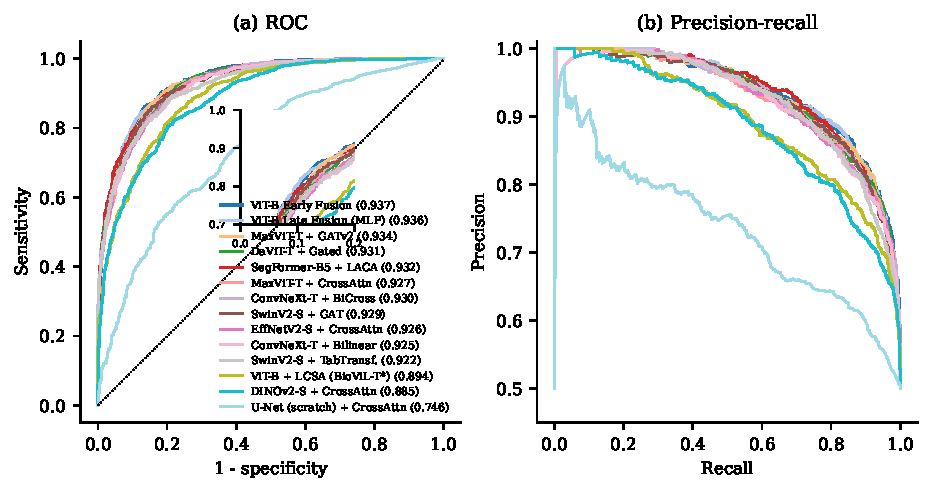
\includegraphics[width=\textwidth]{fig_roc_pr_all}
\caption{(a) ROC and (b) precision--recall curves of all fourteen models on the identical test set ($n=2{,}559$). The legend gives test AUC; the inset magnifies the high-specificity region relevant to screening.}
\label{fig:roc}
\end{figure*}

\begin{figure}[!t]
\centering
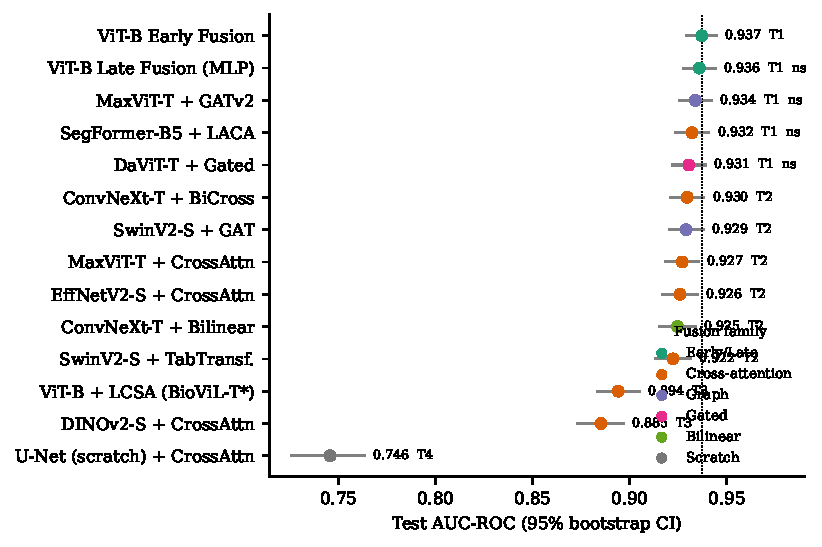
\includegraphics[width=\figw]{fig_auc_forest}
\caption{Test AUC with 95\% bootstrap confidence intervals, coloured by fusion family. T$k$ denotes the statistical tier; \textit{ns}, not significantly different from the best model (Holm-adjusted DeLong).}
\label{fig:forest}
\end{figure}

\begin{figure*}[!t]
\centering
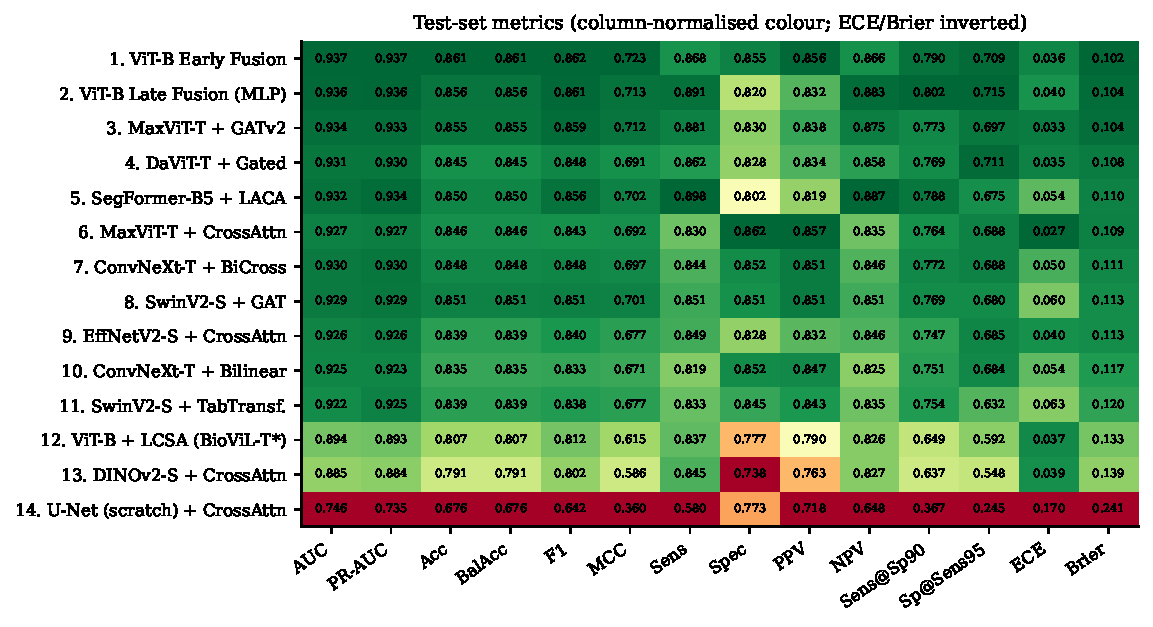
\includegraphics[width=0.85\textwidth]{fig_metric_heatmap}
\caption{Fourteen test metrics for every model (rows ordered by final rank). Colour is column-normalised; ECE and Brier are inverted so that green is always better.}
\label{fig:heat}
\end{figure*}

\begin{figure}[!t]
\centering
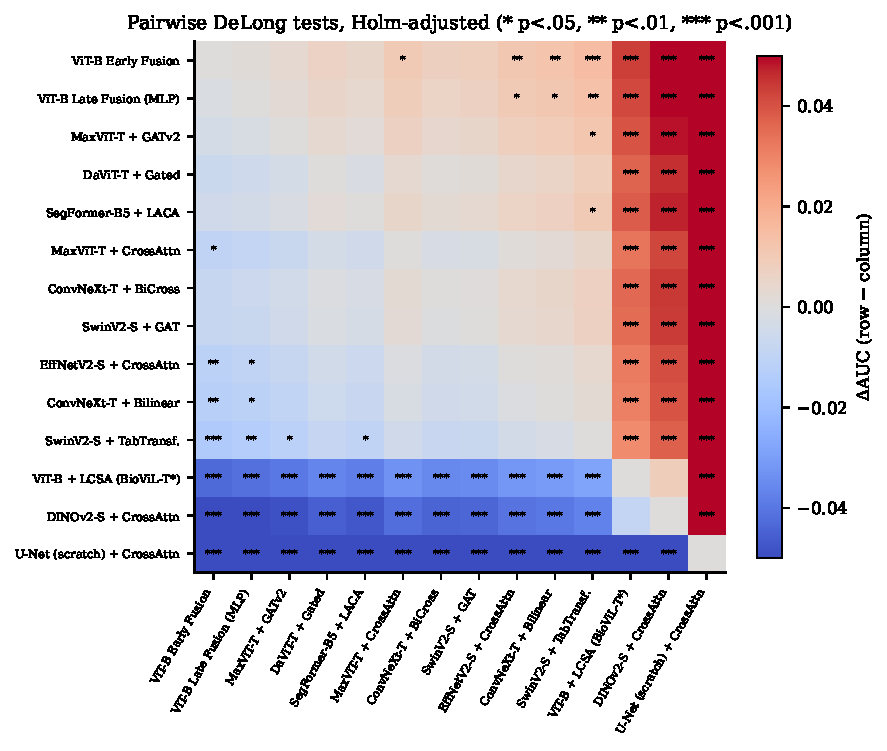
\includegraphics[width=\figw]{fig_delong_pairwise}
\caption{Pairwise AUC differences (row minus column) with Holm-adjusted paired DeLong significance across all 91 model pairs.}
\label{fig:delong}
\end{figure}

\textit{Fusion family versus backbone.} Fusion mechanism explains little of the variance once the backbone is strong (Fig.~\ref{fig:family}). With an identical ViT-B/16 backbone, early token fusion and late concatenation differ by only 0.001 AUC ($p=1.00$). Conversely, holding the TabTransformer cross-attention fusion fixed while changing the backbone spans 0.885 (DINOv2-S) to 0.927 (MaxViT-T), and with Swin-V2-S, replacing cross-attention by graph attention gains 0.007 AUC. Supervised ImageNet pre-training at sufficient capacity, rather than a particular fusion operator, is the primary determinant of performance in this data regime. The scratch U-Net confirms this: its validation AUC peaked at epoch~2 (0.711) and then deteriorated, so training stopped early at epoch~7.

\textit{Operating points.} At the validation-frozen threshold, the leader reaches sensitivity 0.868 and specificity 0.855. At a screening-oriented operating point of 90\% specificity, late-fusion ViT attains the highest sensitivity (0.802), and it also has the best specificity at 95\% sensitivity (0.715). SegFormer-B5+LACA has the highest default-threshold sensitivity (0.898) at a lower specificity (0.802).

\begin{figure*}[!t]
\centering
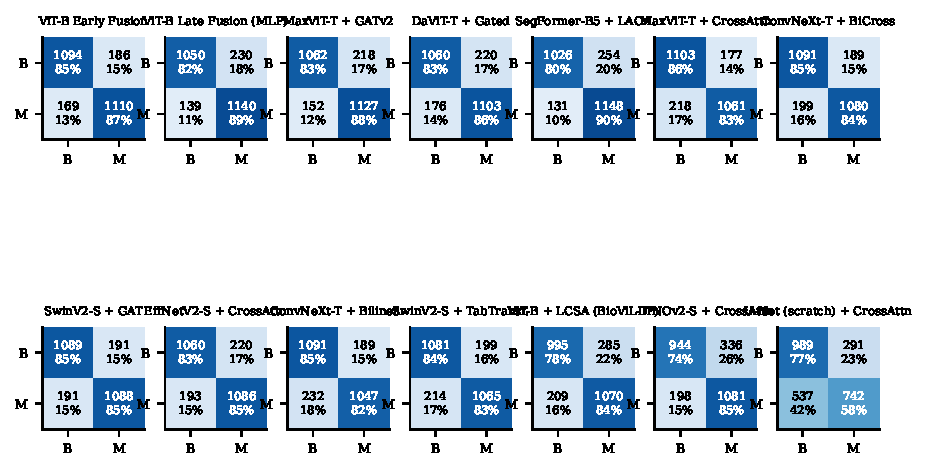
\includegraphics[width=\textwidth]{fig_confusion_all}
\caption{Confusion matrices at each model's validation-frozen threshold (B, benign; M, melanoma), ordered by final rank.}
\label{fig:cm}
\end{figure*}

\subsection{Calibration and Clinical Utility}
After temperature scaling, every pre-trained model is well calibrated (ECE 0.027--0.063; Fig.~\ref{fig:rel}); the learned temperatures range from 1.00 to 1.33, indicating mild over-confidence before scaling. MaxViT-T cross-attention has the lowest ECE (0.027), and MaxViT-T+GATv2 has the lowest ECE in Tier~1 (0.033). The scratch U-Net remains poorly calibrated even after scaling ($T=2.18$, ECE 0.170). In decision-curve analysis (Fig.~\ref{fig:dca}), all Tier~1 models provide a higher net benefit than treat-all and treat-none strategies across threshold probabilities of 0.05--0.8, with near-identical curves, whereas the U-Net is dominated throughout.

\begin{figure*}[!t]
\centering
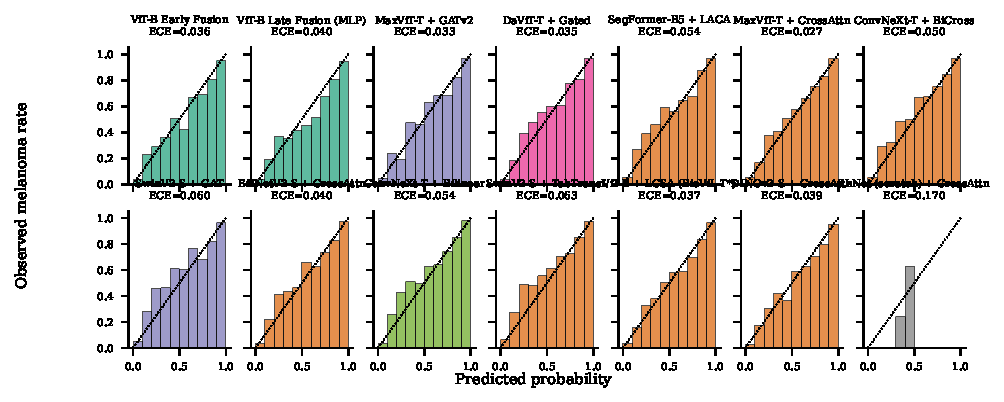
\includegraphics[width=\textwidth]{fig_reliability_all}
\caption{Reliability diagrams after temperature scaling (10 bins) with expected calibration error.}
\label{fig:rel}
\end{figure*}

\begin{figure}[!t]
\centering
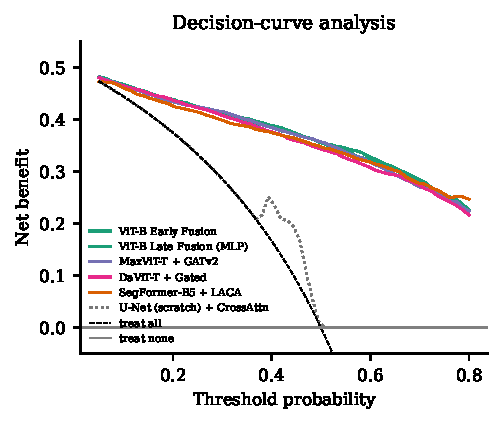
\includegraphics[width=\figw]{fig_decision_curve}
\caption{Decision-curve analysis for the five Tier~1 models and the worst model (dotted).}
\label{fig:dca}
\end{figure}

\begin{figure}[!t]
\centering
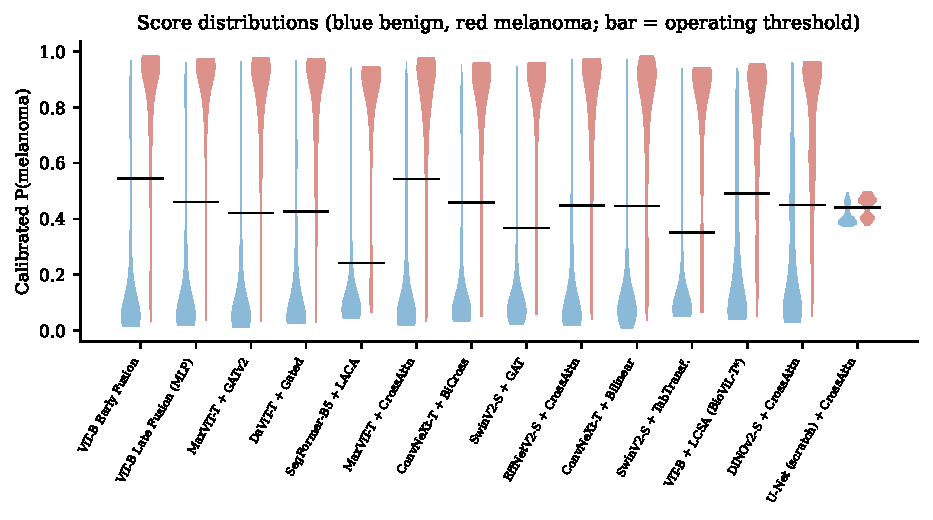
\includegraphics[width=\figw]{fig_prob_violin}
\caption{Distributions of calibrated melanoma probability by true class; the horizontal bar marks each model's operating threshold.}
\label{fig:violin}
\end{figure}

\subsection{Model Agreement, Hard Cases and Ensembling}
Pre-trained models make highly correlated predictions (Fig.~\ref{fig:agree}); pairwise Cohen's $\kappa$ is highest within the Tier~1 group. Across the fourteen models, 1,203 test images (47\%) are classified correctly by every model, and 69 (2.7\%) are misclassified by all of them (Fig.~\ref{fig:diff}). An oracle that is correct whenever any model is correct would reach 97.3\% accuracy, so the errors are only partially redundant. A simple majority vote achieves 85.9\% accuracy, which is no better than the best single model. In contrast, forward selection on validation AUC chose a four-member probability-averaging ensemble (late-fusion ViT, SegFormer-B5+LACA, early-fusion ViT, MaxViT-T+GATv2) that reaches test AUC 0.944 (95\% CI 0.936--0.952), accuracy 0.865 and ECE 0.034, a significant improvement over the best single model (paired DeLong $p<0.001$).

\begin{figure*}[!t]
\centering
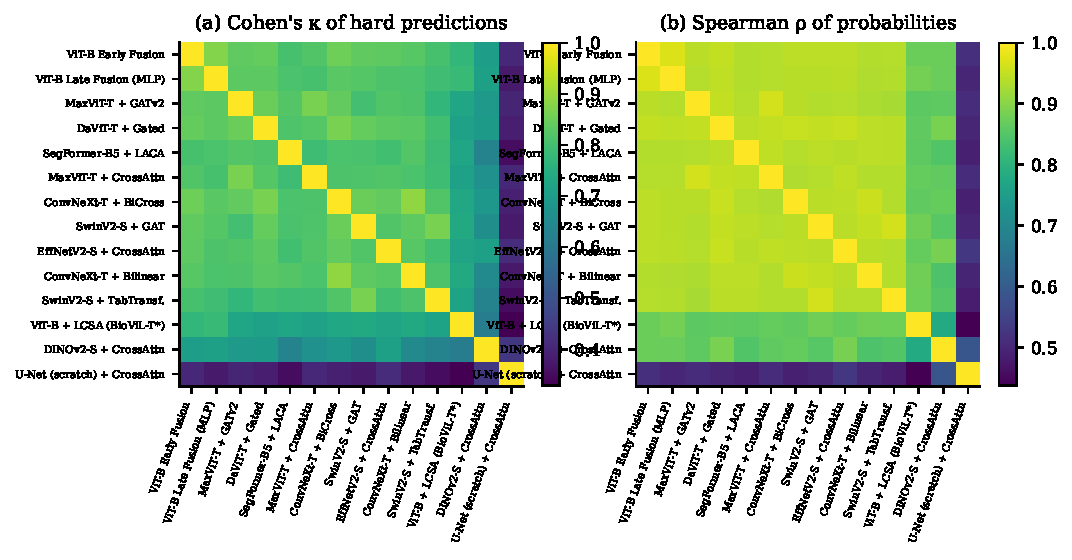
\includegraphics[width=\textwidth]{fig_agreement}
\caption{(a) Cohen's $\kappa$ between hard predictions and (b) Spearman correlation between predicted probabilities for every model pair.}
\label{fig:agree}
\end{figure*}

\begin{figure*}[!t]
\centering
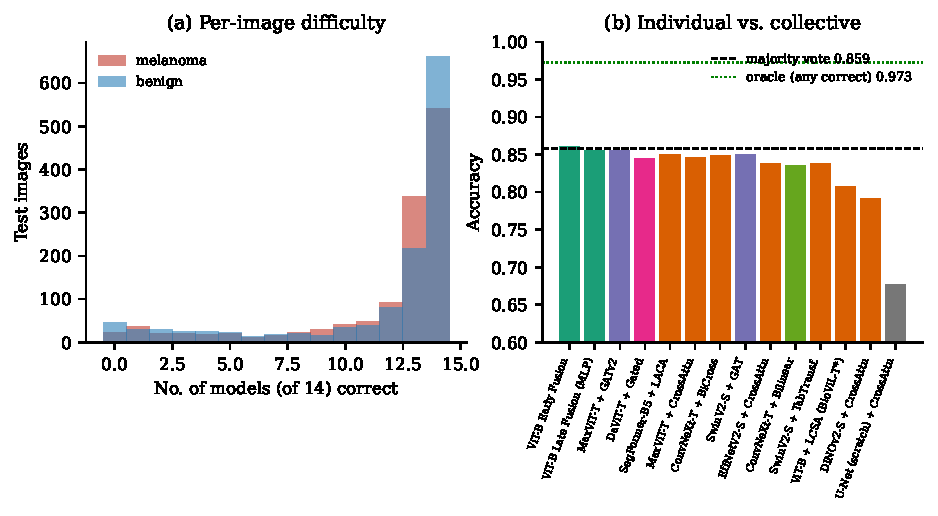
\includegraphics[width=\textwidth]{fig_difficulty}
\caption{(a) Number of models that classify each test image correctly, by class. (b) Individual accuracies compared with majority voting and the any-model-correct oracle.}
\label{fig:diff}
\end{figure*}

\subsection{Robustness: Patient Overlap, Shortcuts and Subgroups}
Fig.~\ref{fig:sub} reports AUC for each subgroup. The largest effect is patient overlap: on the 397 test images from patients unseen in training, the AUC of every model falls, by a median of 0.085 (range 0.013--0.103), to 0.871 for early-fusion ViT, 0.868 for MaxViT-T+GATv2 and 0.865 for late-fusion ViT. Part of this drop reflects a different case mix (melanoma prevalence 36\% versus 53\%), but its magnitude indicates that image-level splits overestimate generalisation to new patients. Importantly, the model ranking is largely preserved on unseen patients (Spearman $\rho=0.83$ with the full-test ranking), so the comparative conclusions stand.

Despite vignette debiasing, all models remain more accurate on vignetted images (early-fusion ViT: AUC 0.977 versus 0.926). Vignetted images are 71\% melanoma in the test set, so residual acquisition bias cannot be excluded. Performance is stable across sex (0.935 versus 0.936), but it is lowest for patients aged 61--85 (0.910), head/neck lesions (0.906) and non-contact polarised dermoscopy (0.857, $n=116$), which are the clinically hardest strata.

\begin{figure*}[!t]
\centering
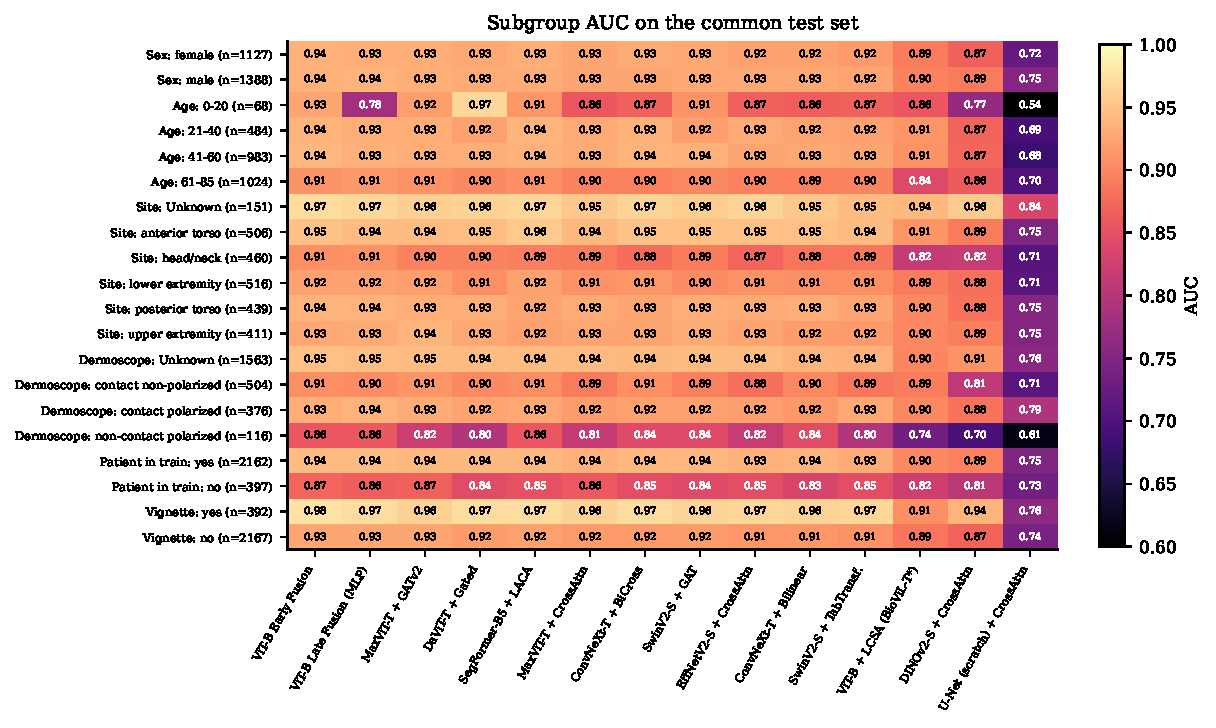
\includegraphics[width=\textwidth]{fig_subgroup_auc}
\caption{Subgroup AUC for every model on the common test set (only subgroups with $n\ge60$ and both classes present are shown). ``Patient in train'' indicates whether the test image's patient also contributes training images.}
\label{fig:sub}
\end{figure*}

\subsection{Efficiency and Training Dynamics}
Fig.~\ref{fig:eff} relates accuracy to model size and training cost. MaxViT-T+GATv2 (31M parameters) and DaViT-T+gated fusion (29M parameters, 21 training minutes) are within 0.004--0.007 AUC of the 86M-parameter ViT-B models, offering the best accuracy--efficiency trade-off for deployment. Seven models reached their best validation AUC in the last two epochs (13--15), which suggests that a larger training budget may yield further gains for the cross-attention and Swin-V2 variants.

\begin{figure*}[!t]
\centering
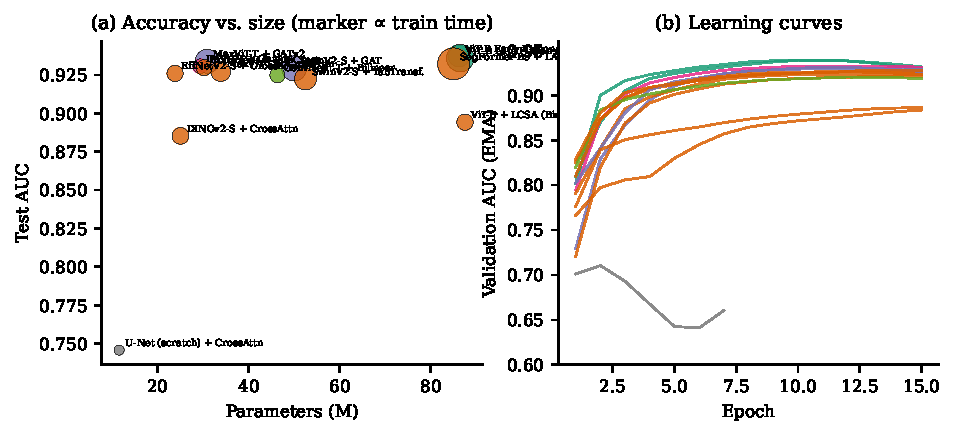
\includegraphics[width=\textwidth]{fig_efficiency_learning}
\caption{(a) Test AUC versus parameter count (marker area is proportional to training time). (b) Validation AUC (EMA weights) per epoch.}
\label{fig:eff}
\end{figure*}

\begin{figure}[!t]
\centering
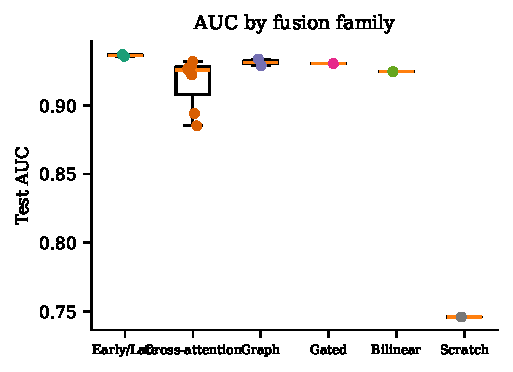
\includegraphics[width=0.8\figw]{fig_family_box}
\caption{Test AUC grouped by fusion family.}
\label{fig:family}
\end{figure}

\subsection{Explainability on Identical Test Cases}
\subsubsection{Qualitative comparison}
Figs.~\ref{fig:xgc}--\ref{fig:xocc} show Grad-CAM, Integrated Gradients and occlusion maps for the same five test images across all fourteen models. For the consensus true positive, every pre-trained model concentrates attribution on the lesion body and its irregular border; the scratch U-Net is undecided ($p=0.48$) and produces diffuse maps. For the consensus true negative and the hardest false negative, a small, faint, light-brown macule that every model scores at $p\le0.08$, Integrated Gradients localises the small lesion consistently, whereas class-activation maps from several hierarchical backbones (Swin-V2, ConvNeXt, DINOv2) spread over the surrounding skin. The hardest false positive is a dark, well-circumscribed, sharply bordered naevus that every pre-trained model scores above 0.86; all attribution methods agree that the decision is driven by the dark pigment network, which indicates a genuine visual mimic rather than an artefact-driven error. On the disputed melanoma, a large lesion extending beyond the field of view with predictions between 0.11 and 0.88, attributions are fragmented and disagree across models, mirroring the model-level uncertainty.

\begin{figure*}[!t]
\centering
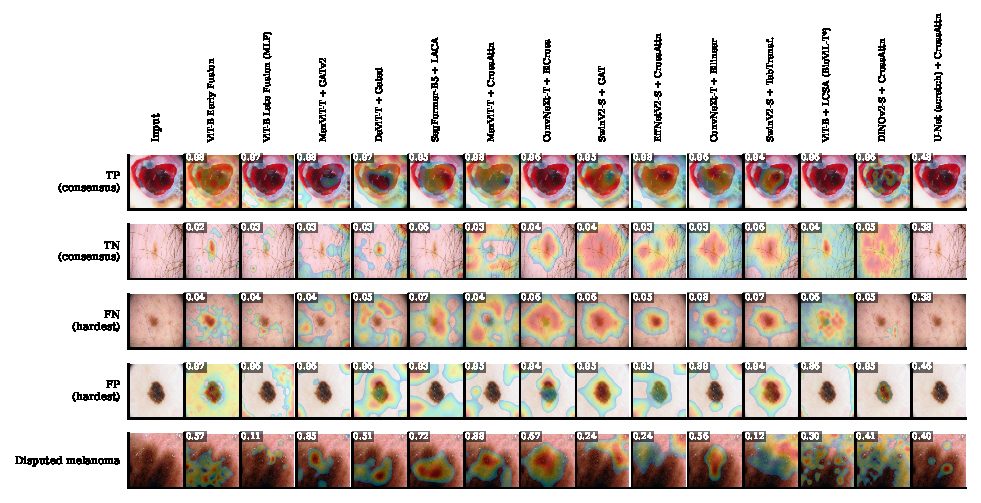
\includegraphics[width=\textwidth]{fig_xai_grid_gradcam}
\caption{Grad-CAM for the predicted class on five identical test images (rows) for all fourteen models (columns, ordered by final rank). The number on each tile is the model's calibrated melanoma probability. Rows: consensus true positive, consensus true negative, hardest false negative, hardest false positive and a disputed melanoma.}
\label{fig:xgc}
\end{figure*}

\begin{figure*}[!t]
\centering
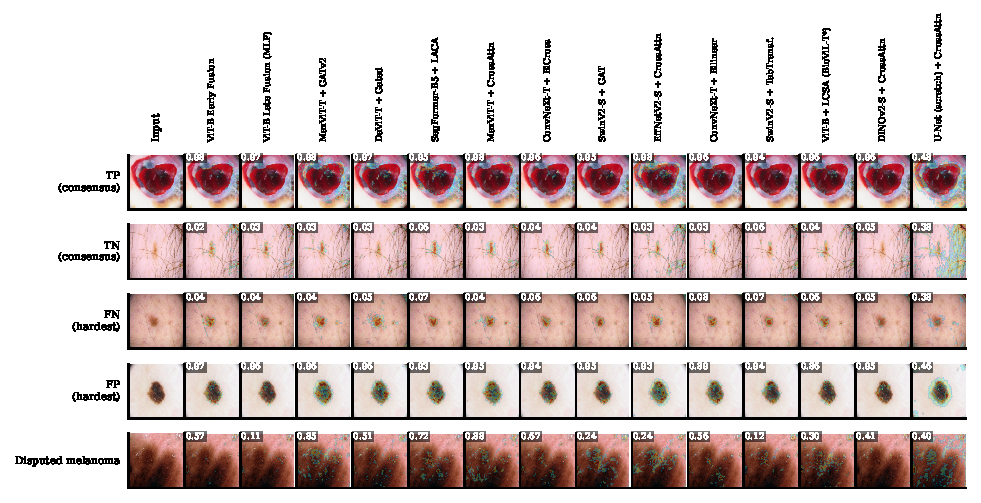
\includegraphics[width=\textwidth]{fig_xai_grid_integrated_gradients}
\caption{Integrated Gradients on the same cases and models as Fig.~\ref{fig:xgc}.}
\label{fig:xig}
\end{figure*}

\begin{figure*}[!t]
\centering
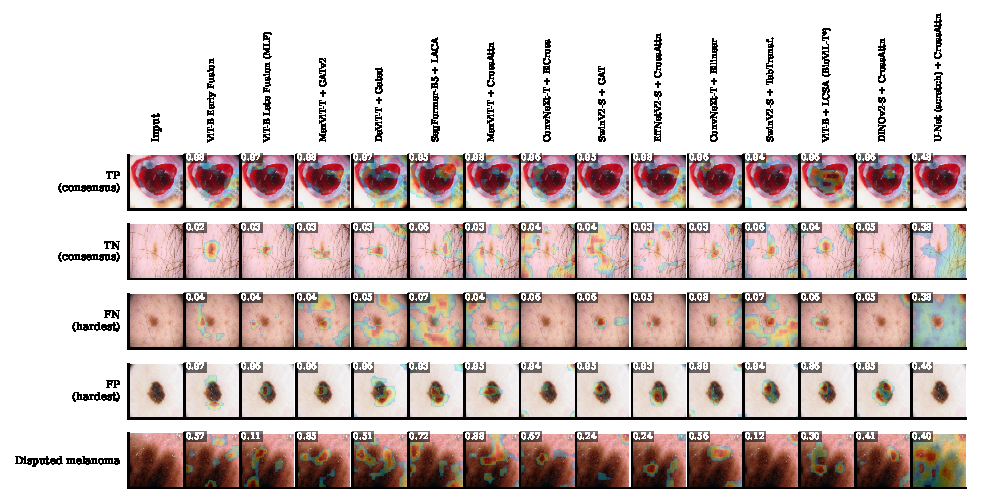
\includegraphics[width=\textwidth]{fig_xai_grid_occlusion}
\caption{Occlusion sensitivity on the same cases and models as Fig.~\ref{fig:xgc}.}
\label{fig:xocc}
\end{figure*}

\subsubsection{Quantitative faithfulness and localisation}
Fig.~\ref{fig:xq} and Table~\ref{tab:xai} summarise the scores on the 32 common evaluation images. Averaged over models, Integrated Gradients is the most faithful method (insertion 0.833, deletion 0.578, gain over random 0.248) and the most lesion-focused (45.1\% of energy inside the lesion, 1.8\% outside the FOV), followed by occlusion (gain 0.211) and gradient-weighted attention roll-out for the ViT encoders (0.187). Grad-CAM (0.142) and especially Grad-CAM++ (0.102) are markedly less faithful: Grad-CAM++ beats the random baseline significantly for only 71\% of the models (Wilcoxon $p<0.05$), compared with 100\% for Integrated Gradients, occlusion and roll-out. The difference between the four methods available for every model is highly significant (Friedman $\chi^2=33.2$, $p=3\times10^{-7}$; Fig.~\ref{fig:xbox}). Architecture-specific signals are weak explanations: the clinical-to-image attention weights of the cross-attention models (gain 0.065) and the LACA gate (0.021) carry little faithful information about the decision, even though they look plausible, so attention weights should not be presented as explanations without such a test.

\begin{table}[!t]
\centering
\caption{Explanation quality averaged over 14 models (32 common test images)}
\label{tab:xai}
\scriptsize
\begin{tabular}{lccccc}
\toprule
Method & Ins.$\uparrow$ & Del.$\downarrow$ & Gain$\uparrow$ & Lesion$\uparrow$ & $>$Rand.\\
\midrule
Integrated Gradients & \textbf{0.833} & \textbf{0.578} & \textbf{0.248} & 0.451 & 100\%\\
Occlusion & 0.809 & 0.592 & 0.211 & 0.375 & 100\%\\
Grad-rollout (ViT) & 0.806 & 0.606 & 0.187 & 0.424 & 100\%\\
Grad-CAM & 0.766 & 0.618 & 0.142 & 0.308 & 93\%\\
Grad-CAM++ & 0.753 & 0.644 & 0.102 & 0.274 & 71\%\\
Clinical$\to$image attn. & 0.707 & 0.649 & 0.065 & 0.348 & 50\%\\
\bottomrule
\multicolumn{6}{p{8cm}}{\footnotesize Gain: (Ins$-$Del) minus that of a smoothed random map. Lesion: fraction of attribution energy inside the lesion mask. $>$Rand.: share of models with a significant gain (Wilcoxon $p<0.05$).}
\end{tabular}
\end{table}

\begin{figure*}[!t]
\centering
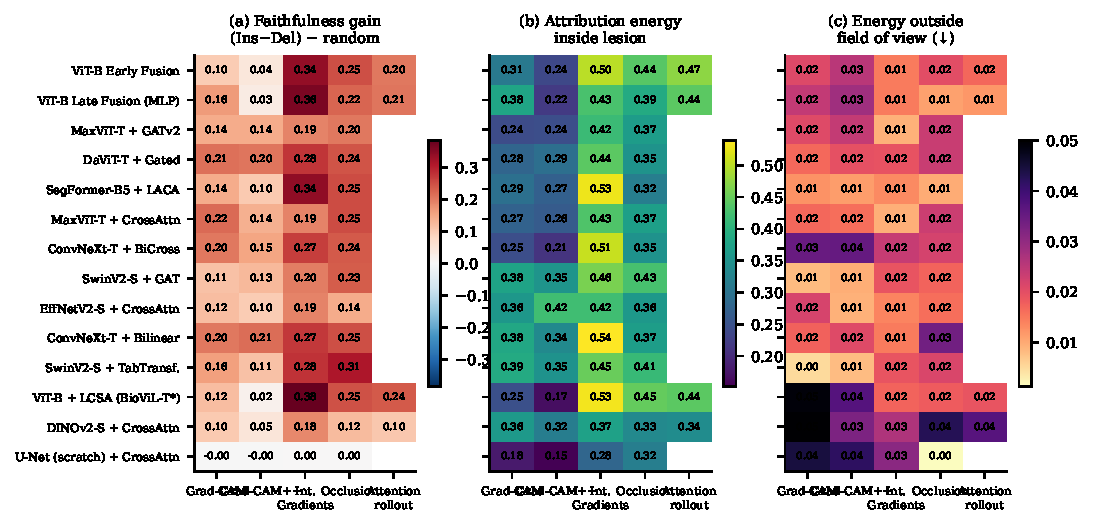
\includegraphics[width=\textwidth]{fig_xai_quant_heatmap}
\caption{Explanation quality per model and method on 32 common test images: (a) faithfulness gain over a random map, (b) attribution energy inside the lesion, (c) energy outside the dermoscope field of view (lower is better).}
\label{fig:xq}
\end{figure*}

\begin{figure}[!t]
\centering
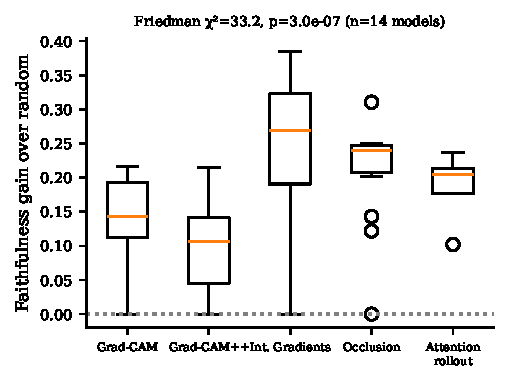
\includegraphics[width=\figw]{fig_xai_method_box}
\caption{Faithfulness gain over random by attribution method; each point set contains one value per model.}
\label{fig:xbox}
\end{figure}

Explanation quality is only weakly related to accuracy. The Spearman correlation between test AUC and Integrated Gradients faithfulness is 0.42, and that between AUC and in-lesion energy is 0.17. The scratch U-Net is the exception: its IG faithfulness gain is zero and only 28\% of its energy falls inside the lesion, consistent with a model that has not learned lesion-level features. Among Tier~1 models, the two ViT-B models and SegFormer-B5 produce the most faithful IG maps (gain 0.34--0.36), whereas MaxViT-T+GATv2 has accurate but less faithful maps (0.19); explanation quality is therefore a useful secondary criterion for selecting among statistically tied models.

\subsubsection{Metadata reliance}
Grouped Shapley values computed on common test images and grouped permutation importance computed on a common 512-image subset agree (Fig.~\ref{fig:meta}). Melanocytic status is the dominant clinical variable (mean $|\phi|=0.093$; permuting it lowers AUC by 0.099 on average), followed by age (0.036; 0.026), anatomical site and dermoscope type; sex and history of melanoma contribute little. Permuting all metadata together lowers AUC by 0.129, which shows that the models genuinely use the clinical branch. The feature rankings are highly concordant across architectures (Kendall's $W=0.74$ for Shapley and 0.73 for permutation importance), which suggests that the learned clinical associations are properties of the data rather than of individual architectures. Unlike the leakage-affected preliminary analysis, no acquisition-protocol variable appears among the top features. Melanocytic status is clinically meaningful (all melanomas are melanocytic), but its strong weight warrants caution because, in the archive metadata, it is itself a coarse diagnostic annotation rather than a patient-reported variable.

\begin{figure*}[!t]
\centering
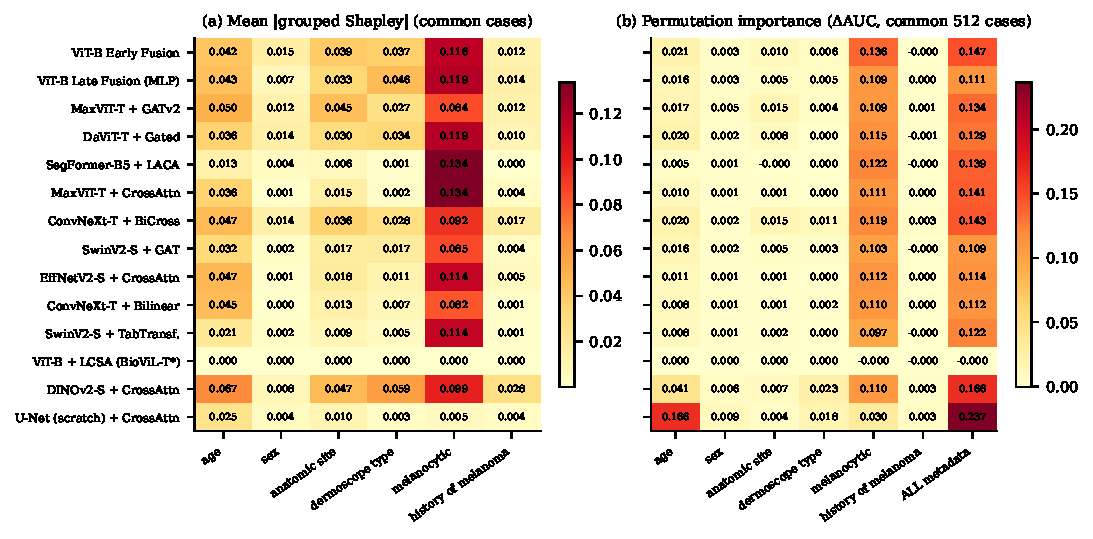
\includegraphics[width=\textwidth]{fig_meta_attribution}
\caption{Metadata reliance of every model: (a) mean absolute grouped Shapley value on common test images; (b) grouped permutation importance (drop in AUC) on a common 512-image subset.}
\label{fig:meta}
\end{figure*}

\section{Discussion}
\textit{Leakage control changes the story.} Our preliminary analysis, like several published multimodal pipelines, included the diagnosis-confirmation field and reported AUC 0.960, with SHAP ranking confirmation type as the most important feature. That pattern is the signature of label leakage rather than clinical insight: the field records how a diagnosis was \emph{obtained}, and benign lesions are disproportionately confirmed without biopsy. Once the field is removed, performance falls to a still strong but more credible 0.937, and the explanations shift to genuine clinical variables. We recommend that multimodal studies on ISIC-derived data report results without acquisition-protocol fields and audit every metadata column for deterministic label associations before training.

\textit{Statistical ties are the norm.} With 2,559 test images, the 95\% CI of a single AUC spans about $\pm0.008$. Five architectures, ranging from 29M to 86M parameters and from gated to graph to token fusion, cannot be separated. Claims that one fusion operator is superior based on third-decimal AUC differences, which are common in the literature, are not supported by paired testing. In our data, choosing a strong pre-trained backbone matters more than the fusion operator: the same cross-attention block spans 0.042 AUC across backbones, while early and late fusion on the same ViT differ by 0.001.

\textit{Ensembling is the reliable gain.} Because errors are only partially shared (oracle accuracy 97.3\%), a small validation-selected ensemble of architecturally diverse Tier~1 models delivers the only statistically significant improvement observed (+0.007 AUC, $p<0.001$), at four times the inference cost. For resource-constrained deployment, MaxViT-T+GATv2 offers near-Tier-1-leader accuracy and the best calibration in its tier at one third of the parameters.

\textit{Generalisation to new patients.} The 84\% patient overlap between the community train and test splits is, to our knowledge, unreported. Lesions from the same patient share skin type, imaging device and photographic conditions, which allows a model to recognise the patient rather than the pathology. The consistent 7--10-point AUC loss on unseen patients indicates that patient-grouped splitting should become standard for ISIC-DICM-17K. The ranking of architectures was stable, but absolute numbers reported on image-level splits, including ours, should be read as optimistic.

\textit{Not all explanations are equal.} Grad-CAM-family maps are the most common explanation in the dermatology literature, yet in our same-case, model-in-the-loop evaluation they were the least faithful, and Grad-CAM++ was frequently indistinguishable from a random map. Path- and perturbation-based attributions (Integrated Gradients, occlusion) were consistently more faithful and more lesion-focused across all fourteen architectures. Attention weights from the fusion modules, which are often presented as intrinsic explanations, carried little decision-relevant information. We therefore recommend reporting at least one perturbation-validated attribution method together with a random-baseline control, and selecting among statistically tied models partly on explanation quality.

\textit{Limitations.} First, the data come from a single archive and predominantly represent lighter Fitzpatrick phototypes; external validation on independent, phototype-diverse cohorts is required. Second, the frozen split is image-level; retraining on a patient-grouped split is the most important next step. Third, each architecture was trained with one seed under a fixed 15-epoch budget; seed variance and longer schedules could reorder models within a tier. Fourth, the lesion masks used for localisation scores are automatically derived rather than expert-annotated. Fifth, faithfulness metrics based on deletion and insertion depend on the perturbation baseline, and no dermatologist user study has yet tested whether these explanations improve clinical decisions.

\section{Ethical and Legal Analysis}
The deployment of AI in clinical diagnostic workflows raises ethical, legal and epistemic concerns that cannot be subordinated to accuracy benchmarks. Under GDPR Article~22 and the EU AI Act, systems that perform automated medical decision-making must provide meaningful explanations, and medical diagnostic AI is classified as high-risk and subject to conformity assessment. Our framework provides visual (saliency) and tabular (Shapley) justifications for each prediction, and, unlike most prior work, it quantifies how faithful those justifications are, which is a prerequisite for an explanation to be meaningful in the legal sense. The system is designed as a decision-support tool that preserves clinicians' final authority.

Algorithmic bias is a second concern. Class balance removes majority-class bias, but our subgroup analysis shows that performance varies by age, anatomical site and imaging device, and phototype information is unavailable. A system that achieves an AUC of 0.94 on the source distribution may perform substantially worse on under-represented populations, so prospective, demographically diverse validation is required before any deployment, in keeping with the principle of distributive justice. The leakage and patient-overlap findings show that dataset curation itself can create unearned performance, which should be disclosed to regulators. Third, clinical liability remains unresolved; transparent, calibrated outputs allow clinicians to exercise informed judgement rather than opaque delegation, reducing but not eliminating this exposure.

\section{Conclusion}
We benchmarked fourteen multimodal fusion architectures for melanoma classification under a single leakage-controlled protocol, on an identical test set, with paired statistical testing and same-case, quantitatively scored explanations. After removing a metadata field that deterministically leaks the label and debiasing a vignette shortcut, ViT-B/16 early fusion ranked first (AUC 0.937, balanced accuracy 0.861, ECE 0.036), but it was statistically tied with four other architectures; backbone pre-training mattered more than fusion design, and a four-model validation-selected ensemble provided a significant improvement (AUC 0.944). An 84\% patient overlap in the community split inflates all absolute results by 7--10 AUC points relative to unseen patients. Faithfulness-scored XAI on identical test cases showed that Integrated Gradients and occlusion are more trustworthy than class-activation maps or fusion attention for these models, and that the models' metadata reliance concentrates on melanocytic status and age, consistently across architectures.
Future work will retrain on a patient-grouped split, validate externally on phototype-diverse cohorts, average over multiple seeds, and evaluate the explanations with dermatologists in a prospective reader study.

\section*{Data and Code Availability}
All code (training, evaluation, unified-case XAI and figure generation), per-model test predictions and result files are available in the project repository. The ISIC-DICM-17K images are publicly available from the ISIC Archive.

\begin{thebibliography}{99}
\bibitem{ahammed2025} S.~Ahammed, X.~Cui, W.~Lu, and M.~H.~Yap, ``Skin lesion classification using dermoscopic images and clinical metadata: Insights from multimodal models,'' in \textit{Proc. IEEE/CVF CVPR Workshops}, 2025, pp.~222--230, doi: 10.1109/CVPRW67362.2025.00027.
\bibitem{kassem2020} M.~A.~Kassem, K.~M.~Hosny, and M.~M.~Fouad, ``Skin lesions classification into eight classes for ISIC 2019 using deep convolutional neural network and transfer learning,'' \textit{IEEE Access}, vol.~8, pp.~114822--114832, 2020.
\bibitem{ahmad2023} N.~Ahmad \textit{et al.}, ``A novel framework of multiclass skin lesion recognition from dermoscopic images using deep learning and explainable AI,'' \textit{Front. Oncol.}, vol.~13, 2023, doi: 10.3389/fonc.2023.1151257.
\bibitem{dosovitskiy2021} A.~Dosovitskiy \textit{et al.}, ``An image is worth 16$\times$16 words: Transformers for image recognition at scale,'' in \textit{Proc. ICLR}, 2021.
\bibitem{raju2025} A.~S.~N.~Raju \textit{et al.}, ``XAI-SkinCADx: A six-stage explainable deep ensemble framework for skin cancer diagnosis and risk-based clinical recommendations,'' \textit{IEEE Access}, vol.~13, pp.~176583--176621, 2025.
\bibitem{metta2024} C.~Metta \textit{et al.}, ``Advancing dermatological diagnostics: Interpretable AI for enhanced skin lesion classification,'' \textit{Diagnostics}, vol.~14, no.~7, p.~753, 2024.
\bibitem{muduli2025} D.~Muduli \textit{et al.}, ``Enhancing skin cancer detection with explainable artificial intelligence: A customized extended deep U-shaped encoder decoder network approach,'' \textit{J. King Saud Univ. Sci.}, vol.~37, 2025.
\bibitem{gamage2024} L.~Gamage \textit{et al.}, ``Melanoma skin cancer identification with explainability utilizing mask guided technique,'' \textit{Electronics}, vol.~13, no.~4, p.~680, 2024.
\bibitem{hong2024} S.~Y.~Hong and L.~P.~Lin, ``Skin lesion classification: A deep learning approach with LIME for explainable AI,'' \textit{JOIV Int. J. Informat. Vis.}, vol.~8, no.~3-2, p.~1536, 2024.
\bibitem{mahmud2025} M.~A.~Mahmud \textit{et al.}, ``Explainable deep learning approaches for high precision early melanoma detection using dermoscopic images,'' \textit{Sci. Rep.}, vol.~15, 2025, doi: 10.1038/s41598-025-09938-4.
\bibitem{ruga2026} T.~Ruga \textit{et al.}, ``MultiExCam: A multi approach and explainable artificial intelligence architecture for skin lesion classification,'' \textit{Comput. Methods Programs Biomed.}, vol.~273, p.~109081, 2026.
\bibitem{aksoy2025} S.~Aksoy, P.~Demircioglu, and I.~Bogrekci, ``Web-based multimodal deep learning platform with XRAI explainability for real-time skin lesion classification and clinical decision support,'' \textit{Cosmetics}, vol.~12, no.~5, p.~194, 2025.
\bibitem{cassidy2020} B.~Cassidy \textit{et al.}, ``The ISIC 2020 challenge dataset: Melanoma classification in dermoscopy,'' arXiv:2008.07360, 2020.
\bibitem{esteva2017} A.~Esteva \textit{et al.}, ``Dermatologist-level classification of skin cancer with deep neural networks,'' \textit{Nature}, vol.~542, pp.~115--118, 2017.
\bibitem{haenssle2018} H.~A.~Haenssle \textit{et al.}, ``Man against machine: Diagnostic performance of a deep learning convolutional neural network for dermoscopic melanoma recognition in comparison to 58 dermatologists,'' \textit{Ann. Oncol.}, vol.~29, no.~8, pp.~1836--1842, 2018.
\bibitem{selvaraju2017} R.~R.~Selvaraju \textit{et al.}, ``Grad-CAM: Visual explanations from deep networks via gradient-based localization,'' in \textit{Proc. IEEE ICCV}, 2017, pp.~618--626.
\bibitem{chattopadhay2018} A.~Chattopadhay, A.~Sarkar, P.~Howlader, and V.~N.~Balasubramanian, ``Grad-CAM++: Generalized gradient-based visual explanations for deep convolutional networks,'' in \textit{Proc. IEEE WACV}, 2018, pp.~839--847.
\bibitem{sundararajan2017} M.~Sundararajan, A.~Taly, and Q.~Yan, ``Axiomatic attribution for deep networks,'' in \textit{Proc. ICML}, 2017, pp.~3319--3328.
\bibitem{zeiler2014} M.~D.~Zeiler and R.~Fergus, ``Visualizing and understanding convolutional networks,'' in \textit{Proc. ECCV}, 2014, pp.~818--833.
\bibitem{ribeiro2016} M.~T.~Ribeiro, S.~Singh, and C.~Guestrin, ```Why should I trust you?': Explaining the predictions of any classifier,'' in \textit{Proc. ACM SIGKDD}, 2016, pp.~1135--1144.
\bibitem{lundberg2017} S.~M.~Lundberg and S.-I.~Lee, ``A unified approach to interpreting model predictions,'' in \textit{Proc. NeurIPS}, 2017, pp.~4765--4774.
\bibitem{petsiuk2018} V.~Petsiuk, A.~Das, and K.~Saenko, ``RISE: Randomized input sampling for explanation of black-box models,'' in \textit{Proc. BMVC}, 2018.
\bibitem{adebayo2018} J.~Adebayo \textit{et al.}, ``Sanity checks for saliency maps,'' in \textit{Proc. NeurIPS}, 2018, pp.~9505--9515.
\bibitem{geirhos2020} R.~Geirhos \textit{et al.}, ``Shortcut learning in deep neural networks,'' \textit{Nat. Mach. Intell.}, vol.~2, pp.~665--673, 2020.
\bibitem{winkler2019} J.~K.~Winkler \textit{et al.}, ``Association between surgical skin markings in dermoscopic images and diagnostic performance of a deep learning convolutional neural network for melanoma recognition,'' \textit{JAMA Dermatol.}, vol.~155, no.~10, pp.~1135--1141, 2019.
\bibitem{bissoto2019} A.~Bissoto, M.~Fornaciali, E.~Valle, and S.~Avila, ``(De)constructing bias on skin lesion datasets,'' in \textit{Proc. IEEE/CVF CVPR Workshops}, 2019.
\bibitem{delong1988} E.~R.~DeLong, D.~M.~DeLong, and D.~L.~Clarke-Pearson, ``Comparing the areas under two or more correlated receiver operating characteristic curves: A nonparametric approach,'' \textit{Biometrics}, vol.~44, no.~3, pp.~837--845, 1988.
\bibitem{holm1979} S.~Holm, ``A simple sequentially rejective multiple test procedure,'' \textit{Scand. J. Statist.}, vol.~6, no.~2, pp.~65--70, 1979.
\bibitem{guo2017} C.~Guo, G.~Pleiss, Y.~Sun, and K.~Q.~Weinberger, ``On calibration of modern neural networks,'' in \textit{Proc. ICML}, 2017, pp.~1321--1330.
\bibitem{vickers2006} A.~J.~Vickers and E.~B.~Elkin, ``Decision curve analysis: A novel method for evaluating prediction models,'' \textit{Med. Decis. Making}, vol.~26, no.~6, pp.~565--574, 2006.
\end{thebibliography}

\end{document}
